\chapter{State of the art}
    \section{Windows Subsystem for Linux}
        \subsection{WSL Main Components}
            \begin{figure}[H]
                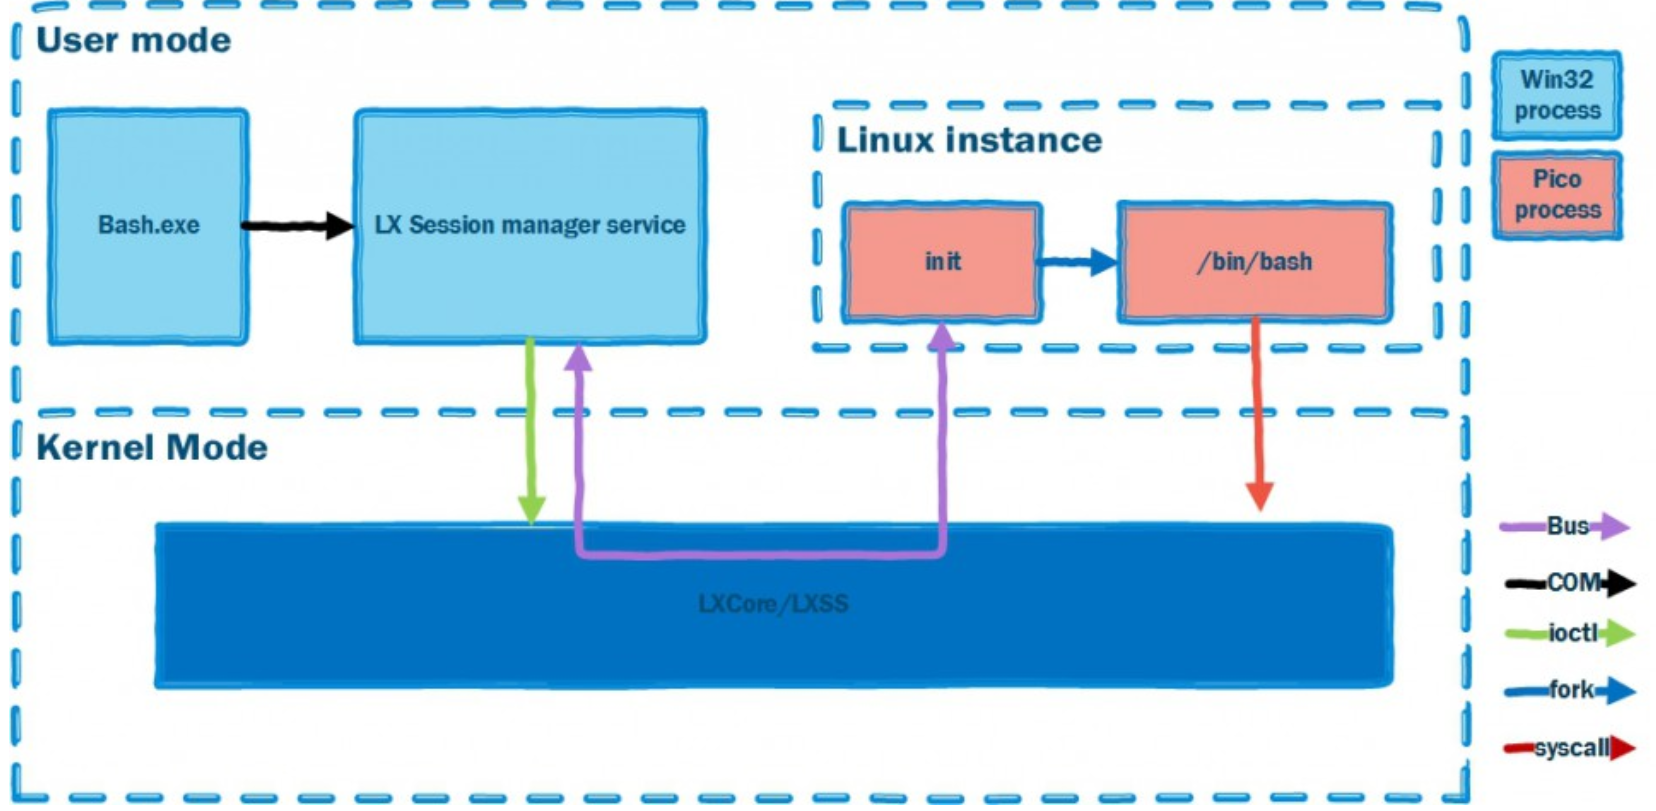
\includegraphics[width=\linewidth]{img/wsl_components.png}
                \caption{WSL Compoents \protect\cite{wslcomponents}}
                \label{fig:wsl_components}
            \end{figure}

        \subsection{WSL File System}
            \begin{figure}[H]
                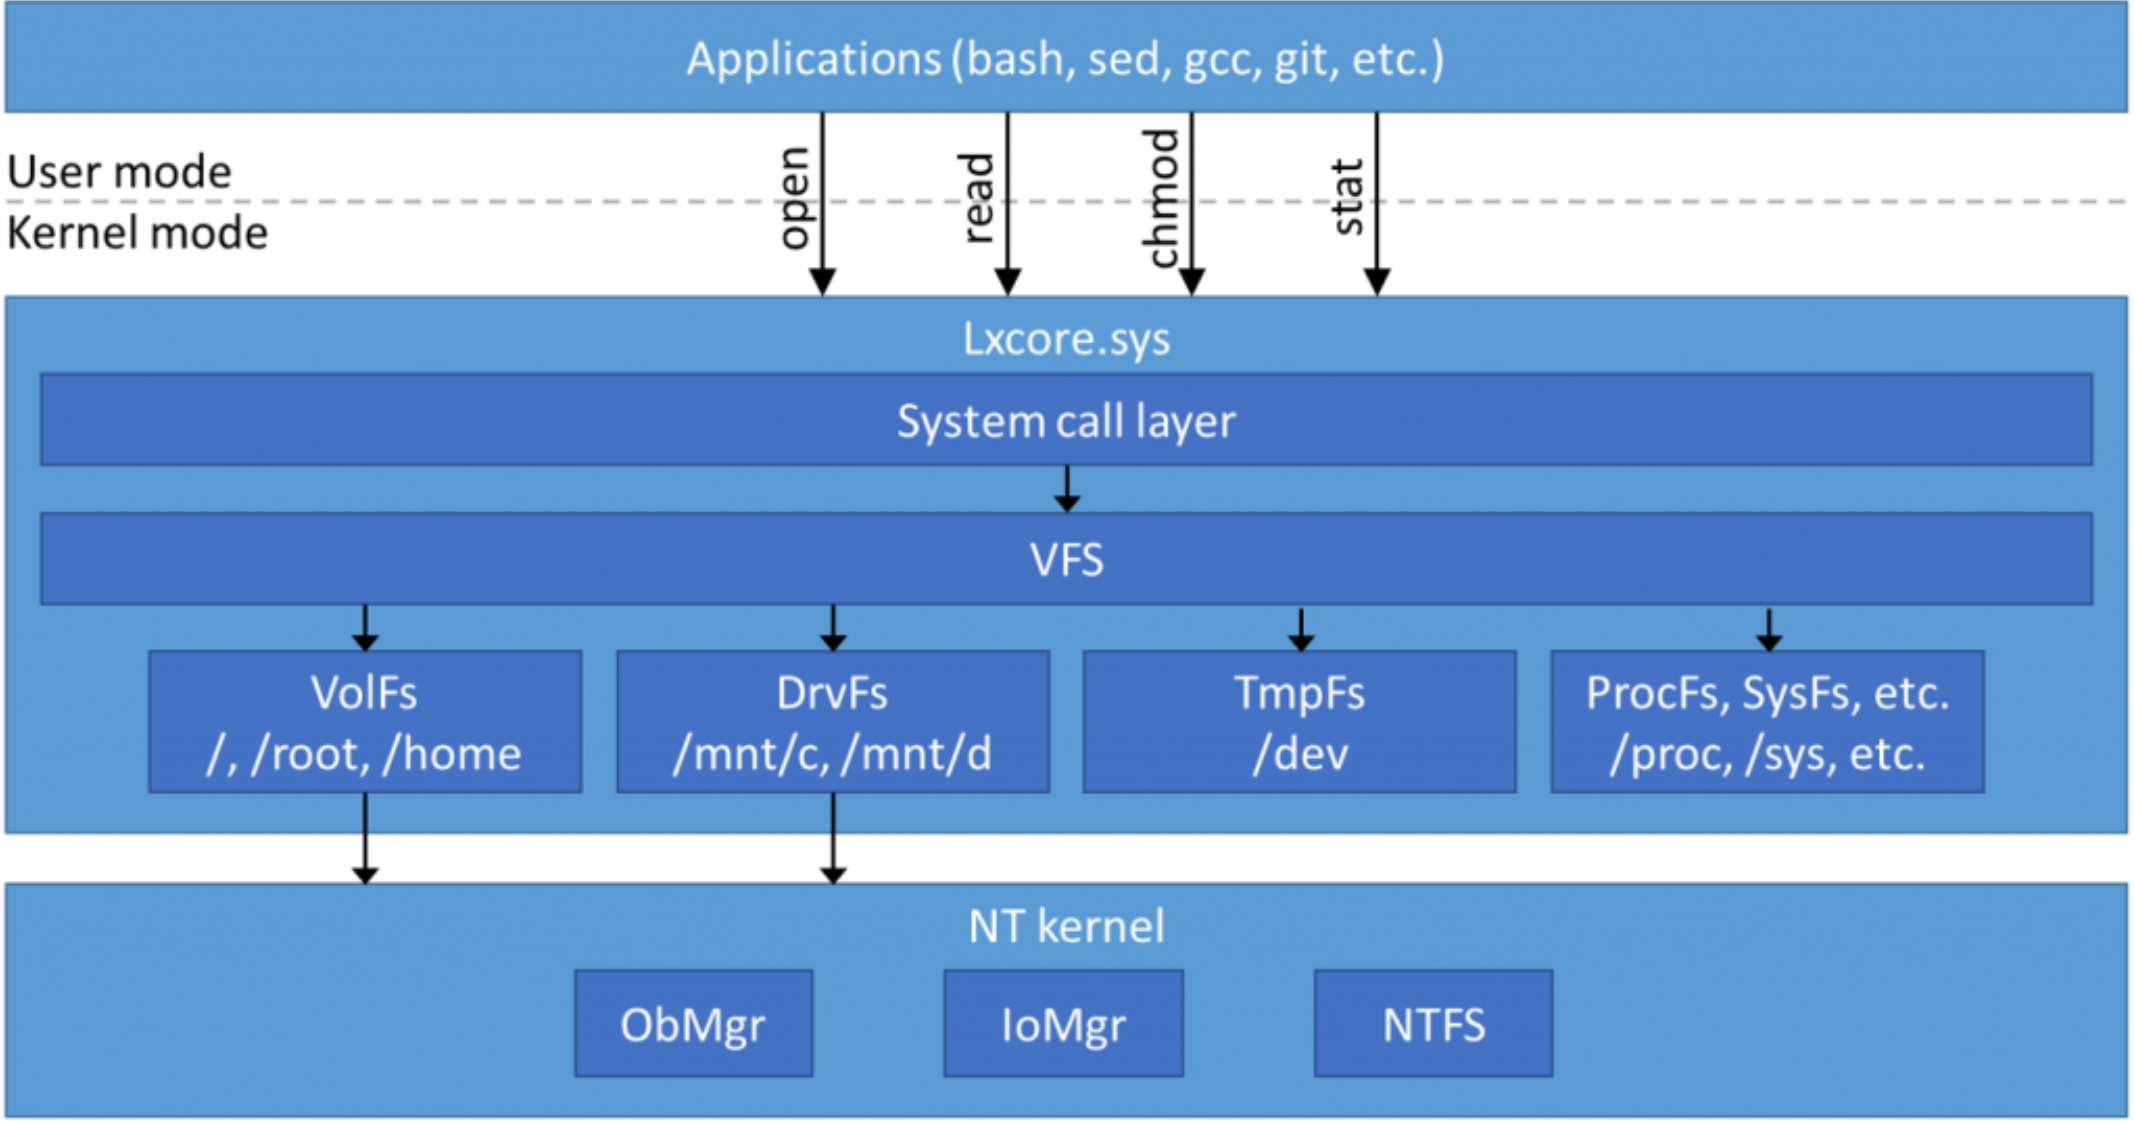
\includegraphics[width=\linewidth]{img/wsl_file_system.png}
                \caption{WSL File System \protect\cite{wslfilesystem}}
                \label{fig:wsl_file_system}
            \end{figure}

        
        \subsection{Security Issues}
        
        
    \section{Bashware and Exploits}
        \paragraph{}
        Bashware is a type of malware that leverages WSL in order to bypass monitoring tools and anti-virus products in order to do damage to the
        operating system.
        
        \subsection{execve exploit}
            \paragraph{}
            Discovered in February 2018 by Saar Amar, security researcher, is a privilege escalation exploit that leverages a vulnerability in
            lxcore, more exactly an integer overflow in LxpUtilReadUserStringSet. Starting from this vulnerability, the exploit proof of concept
            copies the system security descriptor over another process' security descriptor, elevating it at runtime.

        \subsection{File Infector}
            \paragraph{}
            A wsl file infector would essentially inject into windows executable files, altering the code in order to deliver some malicious
            code.
            
        \subsection{Local Denial of Service}
            \paragraph{}
            While experimenting with Event Tracing for Windows (ETW) I've found a way of consistently cause lxcore.sys to run into a Blue Scren
            of Death (BSOD), due to an access violation exception. This can be triggerd from a normal process with no admin rights. I will not
            go into more detail about this yet, as it would not respect the responsible disclore policy, since it wasn't yet fixed by Microsoft.
            Releasing information about how to trigger this local denial of service attack could cause exploitation in the wild.

    \section{Behavioral Detection}
        \paragraph{}
        